% Bioinformatics Application Note -- dicaros
% Self-contained: compiles with pdflatex + bibtex (no journal .cls required).
% To submit, the body can be dropped into the official OUP/Bioinformatics
% LaTeX template; structure and length (<=4 pages) already follow the journal's
% Application Note guidelines.
\documentclass[twocolumn,10pt]{article}

\usepackage[utf8]{inputenc}
\usepackage[T1]{fontenc}
\usepackage{times}
\usepackage{graphicx}
\usepackage{amsmath,amssymb}
\usepackage{booktabs}
\usepackage[margin=2cm]{geometry}
\usepackage{xcolor}
\usepackage[colorlinks=true,linkcolor=blue,citecolor=blue,urlcolor=blue]{hyperref}
\usepackage{authblk}
\usepackage[round]{natbib}
\usepackage{caption}
\captionsetup{font=small,labelfont=bf}

\setlength{\parskip}{2pt}
\renewcommand{\baselinestretch}{1.02}

\title{\vspace{-1.5em}\textbf{DICAROS: Diffeomorphic Ancestral Shape
Reconstruction on Phylogenies}\vspace{-0.5em}}

\author[1]{Michael Lind Severinsen\textsuperscript{*}}
\author[2]{Jacky Kaiyuan Li\thanks{These authors contributed equally. Corresponding author: \texttt{li\_jacky@berkeley.edu}}}
\author[3]{Wonseop Lim}
\author[3]{Levi Yoder Raskin}
\author[4]{Gefan Yang}
\author[4]{Stefan Sommer}
\author[5]{Christy Anna Hipsley}
\author[1,3,6]{Rasmus Nielsen}

\affil[1]{\small GeoGenetics Centre, Globe Institute, University of Copenhagen, Copenhagen 1350, Denmark}
\affil[2]{\small Biostatistics Division, University of California, Berkeley, CA 94720, USA}
\affil[3]{\small Department of Integrative Biology, University of California, Berkeley, CA 94720, USA}
\affil[4]{\small Department of Computer Science, University of Copenhagen, Copenhagen 1350, Denmark}
\affil[5]{\small Department of Biology, University of Copenhagen, Copenhagen 2200, Denmark}
\affil[6]{\small Department of Statistics, University of California, Berkeley, CA 94720, USA}
\date{}


\begin{document}
\twocolumn[
  \begin{@twocolumnfalse}
    \maketitle
    \vspace{-1.5em}
    \begin{abstract}
    \noindent
    \textbf{Summary:} Reconstructing ancestral morphology on a phylogeny is a central task in evolutionary morphometrics. Established reconstruction methods, including multivariate Brownian-motion approaches, rely on linear assumptions and do not directly model the correlations between landmarks within a shape, which can oversimplify the reconstructed morphology. The DICAROS method---Diffeomorphic Independent Contrasts for Ancestral Reconstruction of Shapes \citep{severinsen2026dicaros}---instead fuses sibling shapes along branches with large-deformation diffeomorphic (LDDMM) landmark dynamics that model these correlations, so that ancestors stay on the shape manifold; it was shown to outperform ordinary least-squares, Brownian-motion, and penalized-likelihood reconstruction, particularly on non-symmetric trees. \texttt{dicaros} repackages that pipeline as a documented, pip-installable tool that runs on arbitrary landmark datasets from a single command. It handles 2D and 3D landmarks, Newick and NEXUS trees, a choice of Euclidean or Fréchet species means, optional anchor-based alignment, and tips backed by a single specimen, and it returns the reconstructed shapes for all nodes together with the tree relabelled at its internal nodes. We demonstrate it on two new datasets---a 2D leaf dataset (217 species) and a 3D guenon skull dataset (22 species).

    \noindent\textbf{Availability and Implementation:} \texttt{dicaros} is a pip-installable Python package, freely available without registration under the MIT license at \url{https://github.com/MichaelSev/DICAROS}, with the two example datasets, documentation and reproduction scripts.

    \noindent\textbf{Contact:} \href{mailto:li_jacky@berkeley.edu}{li\_jacky@berkeley.edu}

    \noindent\textbf{Supplementary information:} Supplementary data (CPU and GPU
    runtime benchmarks) are available at \textit{Bioinformatics} online.
    \end{abstract}
    \vspace{1em}
  \end{@twocolumnfalse}
]

\section{Introduction}
Geometric morphometrics summarizes biological form as configurations of homologous landmarks, and a recurring question is what the form of an ancestor looked like, given the forms of its descendants and a phylogeny \citep{bookstein1991morphometric,adams2018phylomorphospace}. Ancestral shapes are routinely reconstructed by fitting an evolutionary model to Procrustes-aligned landmark coordinates---by ordinary least squares, by maximum likelihood under Brownian motion, or by penalized likelihood \citep{slater2012ancestral,adams2013geomorph,revell2012phytools}---and multivariate formulations explicitly account for the covariance among coordinates \citep{clavel2015mvmorph}. These approaches rely on linear assumptions in the Procrustes-aligned (Kendall) shape space and do not directly model the correlations between landmarks within a shape \citep{severinsen2026dicaros}; even when among-coordinate covariance is included, the curved geometry of shape space is only linearly approximated, so reconstructed ancestral morphologies can be oversimplified.

A geometric alternative is to model the transition between two shapes as a smooth deformation (a diffeomorphism) and to reconstruct ancestors as shapes that lie on geodesics between their descendants, using the large-deformation diffeomorphic metric mapping (LDDMM) framework for landmarks \citep{joshi2000landmark,younes2010shapes}. \citet{severinsen2026dicaros} implemented this as the DICAROS (Diffeomorphic Independent Contrasts for Ancestral Reconstruction of Shapes) method, which combines LDDMM landmark dynamics with Felsenstein's phylogenetic independent contrasts \citep{felsenstein1985} and, validated on swallowtail butterfly wings, outperformed ordinary least-squares, Brownian-motion, and penalized-likelihood reconstruction in accuracy---particularly on non-symmetric trees, with comparable accuracy on symmetric ones. \texttt{dicaros} repackages the same pipeline as a documented, \texttt{pip}-installable tool that applies to arbitrary 2D and 3D landmark datasets from a single command, lowering the barrier to using the method.

\section{Methods}
\paragraph{Per-species means.} Each individual specimen row is assigned to a species (a tip). Specimens within a species are Procrustes-superimposed \citep{gower1975generalized,rohlf1990procrustes} and reduced to a single mean shape, either the ordinary Euclidean mean, or the Fréchet (Karcher) mean on the LDDMM landmark manifold; the species means are then aligned into one common frame. Alignment uses all landmarks by default, or only a user-supplied subset of anchor landmarks (\texttt{idxs}) when a few homologous points should define the frame. When a species is represented by a single specimen, that specimen is used directly as the tip mean, and a warning naming the tip is emitted, so the reconstruction proceeds rather than failing.

\paragraph{DICAROS reconstruction.} The reconstruction follows \citet{severinsen2026dicaros}: a single leaves-to-root message pass over a rooted, bifurcating tree (built on \texttt{hyperiax}; \citealp{hyperiax}). At each internal node, the two child shapes are fused on the landmark manifold (using \texttt{jaxgeometry}; \citealp{jaxgeometry}): the shorter child branch defines a base point, the Riemannian logarithm toward the other child gives a momentum (a diffeomorphic independent contrast), and the Hamiltonian geodesic is integrated to the point along the branch fixed by the relative branch lengths. The fused estimate becomes the node's shape, and the pass continues to the root,
so every ancestor is itself a valid shape on the landmark manifold rather than a linear interpolation of coordinates. In \texttt{dicaros}, the Gaussian kernel width $\sigma$ that sets the spatial correlation between landmarks is taken from the mean nearest-neighbor landmark spacing, so it matches the data scale.

\paragraph{Inputs and outputs.} Landmark tables are plain CSV; coordinate columns are selected by regex, start index, or explicit list, accommodating
arbitrary leading metadata columns. Trees may be Newick or NEXUS, including 10kTrees-style \texttt{translate} tables \citep{arnold2010tenktrees}, and are pruned to the species present in the data, with polytomies arbitrarily resolved with very small branch lengths. The output is (i)~a CSV of reconstructed landmark configurations for \emph{all} nodes (tips
and ancestors), and (ii)~the input tree with internal nodes labeled, so each CSV row maps back onto the phylogeny. Implementation is in Python on top of JAX
\citep{jax2018github}; the diffeomorphic step runs on CPU by default.

\section{Usage and examples}
From the command line:
{\footnotesize
\begin{verbatim}
dicaros --landmarks leaves.csv --tree tree.nwk \
        --dim 2 --species-col species \
        --landmark-regex '^[xy][0-9]+$' \
        --output-dir out/leaf
\end{verbatim}}
\noindent or equivalently through the \texttt{dicaros.reconstruct(...)} Python function. The user chooses the mean estimator (\texttt{--mean euclidean|frechet}) and whether to anchor alignment on specific landmarks (\texttt{--idxs}).

Whereas DICAROS was originally validated on swallowtail butterfly wings \citep{severinsen2026dicaros}, we applied \texttt{dicaros} to two further, contrasting datasets (Table~\ref{tab:results}): a 2D dataset of 102-landmark grass (Poaceae) leaf outlines for 217 species \citep{gallaher2019leaf,gallaher2019dryadleaf}, and a 3D dataset of 155-landmark guenon skulls for 22 species \citep{cardini2017wainer} on the 10kTrees primate phylogeny \citep{arnold2010tenktrees}. The leaf dataset includes 17 single-specimen tips, and the guenon dataset includes one, all handled automatically. For each dataset \texttt{dicaros} reconstructs a shape at every ancestral node; Figure~\ref{fig:results} shows the resulting phylomorphospaces (a principal-component ordination of all node shapes with the tree edges drawn in shape space) and the reconstructed root overlaid on the tip means.

\begin{table}[t]
\centering
\caption{Reconstruction on the two bundled datasets. Ancestors $=$ internal nodes reconstructed; singletons $=$ tips backed by one specimen.}
\label{tab:results}
\resizebox{\columnwidth}{!}{%
\begin{tabular}{lccccc}
\toprule
Dataset & Dim & Tips & Ancestors & Landmarks & Singletons \\
\midrule
Leaves          & 2D & 217 & 216 & 102 & 17 \\
Guenon skulls   & 3D & 22  & 21  & 155 & 1  \\
\bottomrule
\end{tabular}}
\end{table}

\begin{figure*}[t]
\centering
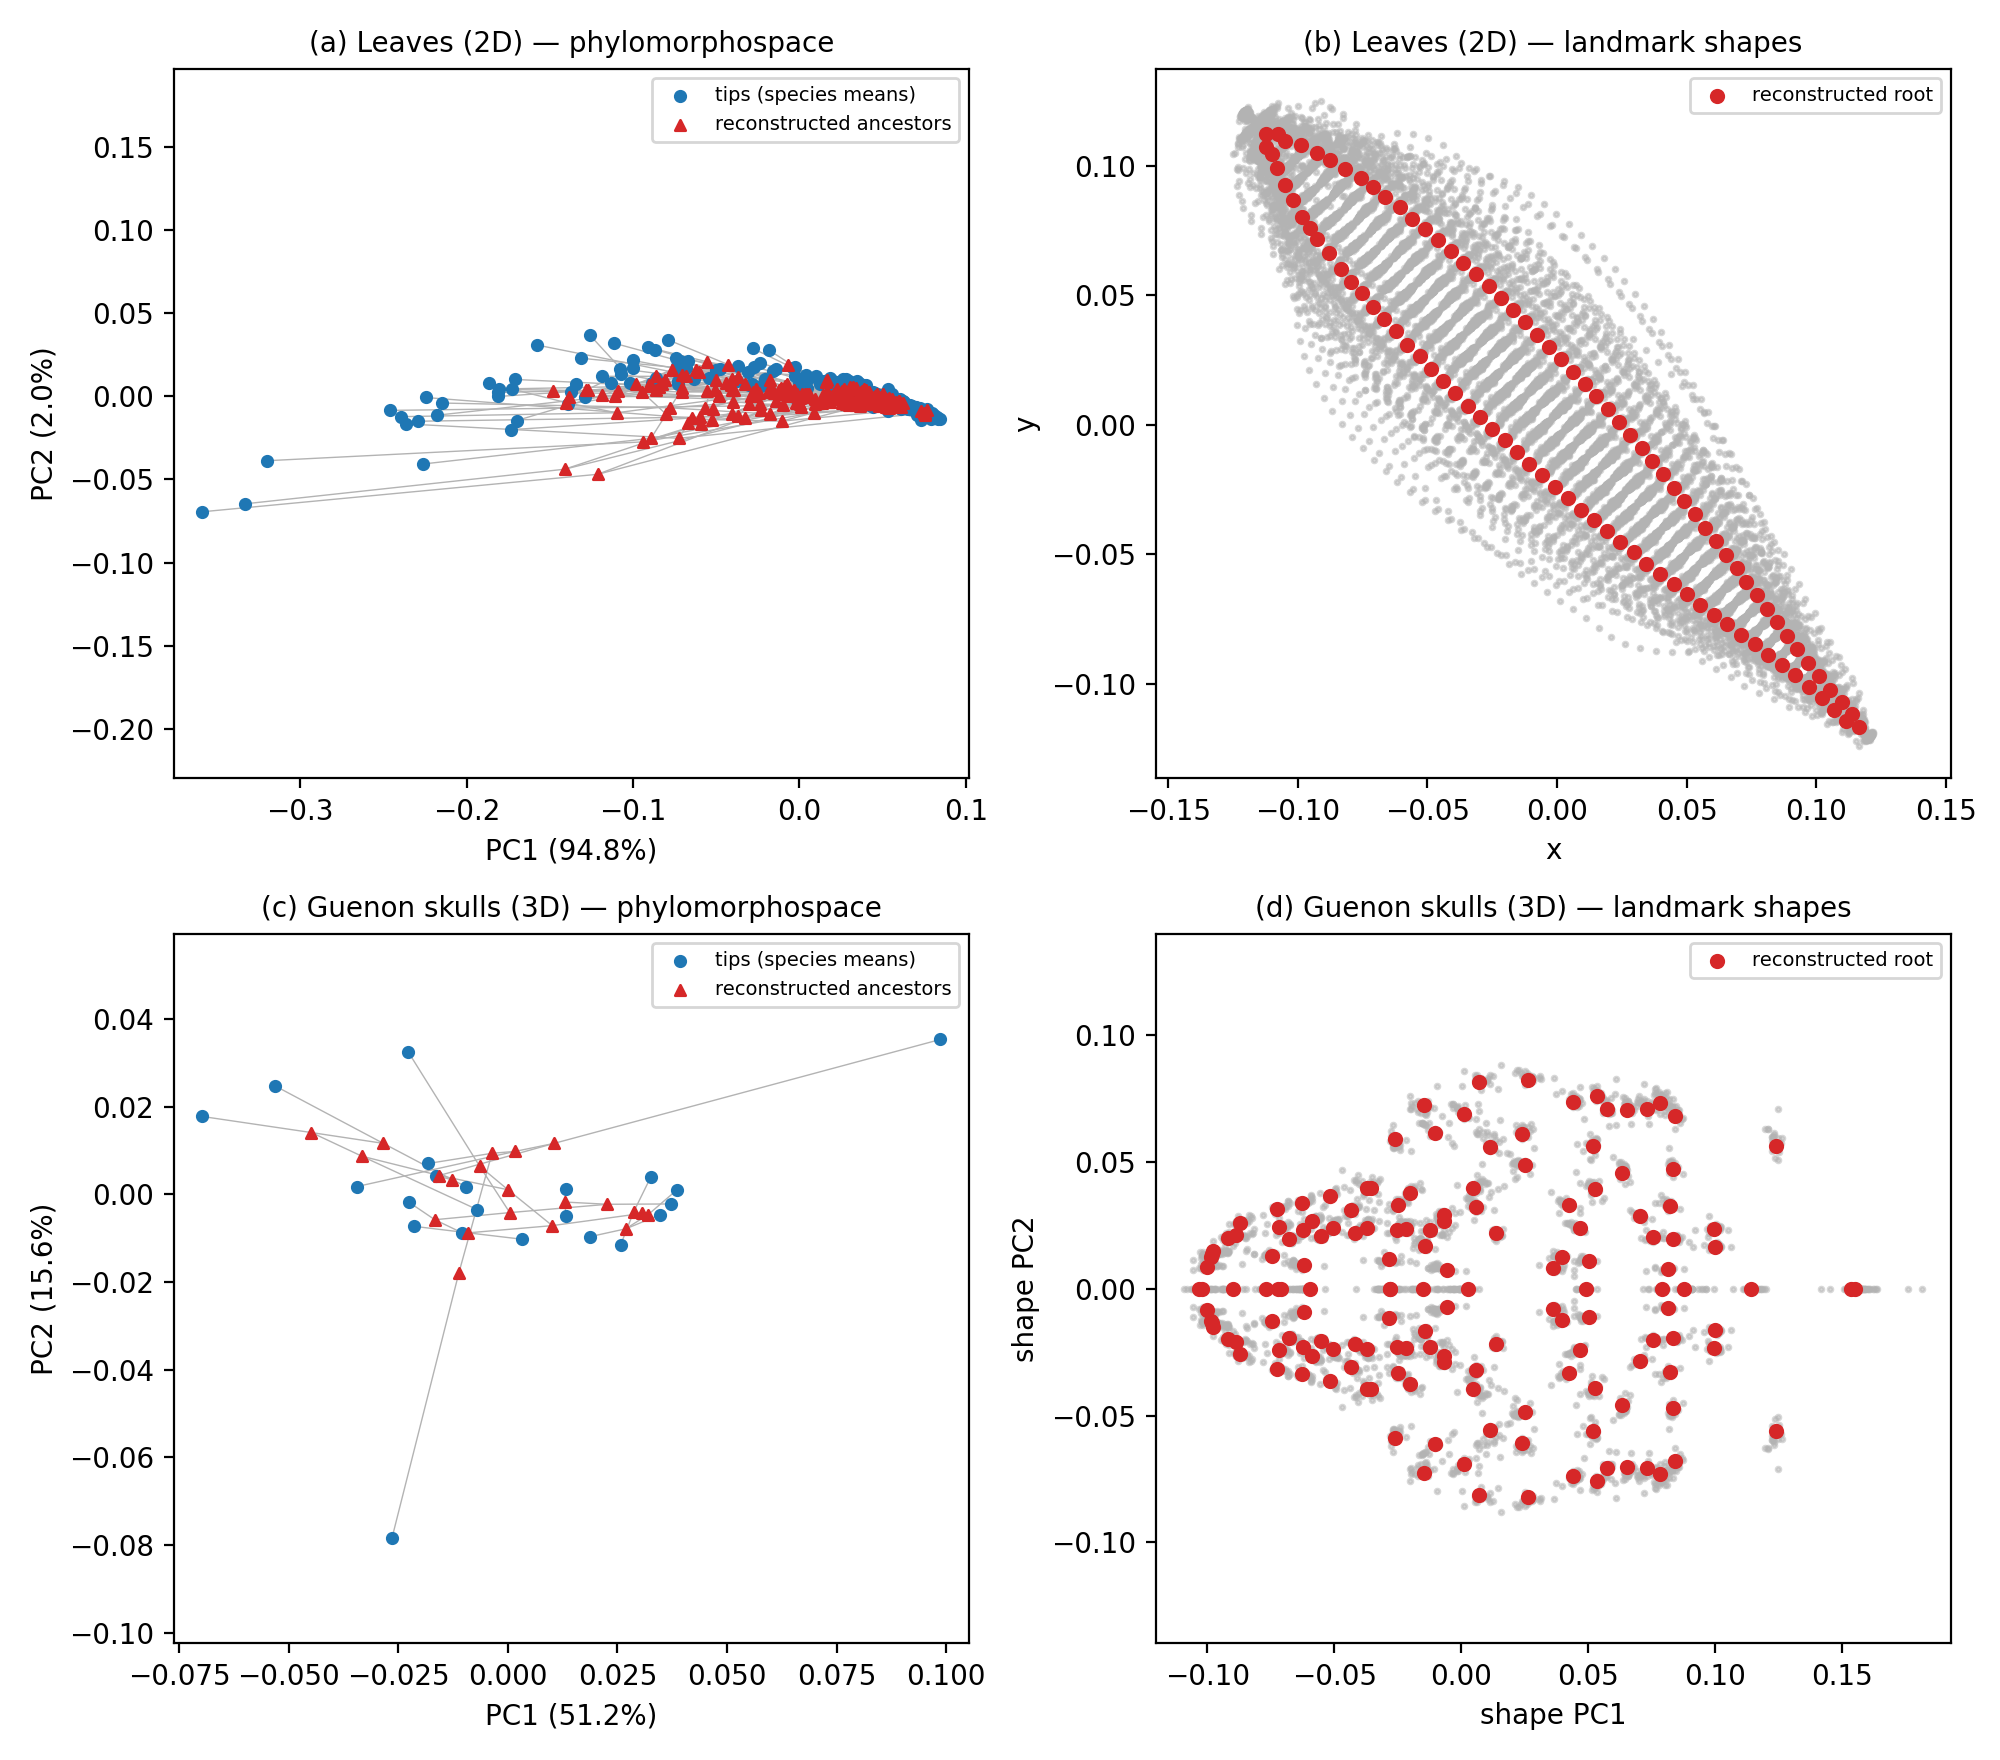
\includegraphics[width=0.66\textwidth]{figures/dicaros_results.png}
\caption{Reconstruction on the two example datasets. Top, leaf dataset (2D, 217
species); bottom, guenon skull dataset (3D, 22 species). (a,c)~Phylomorphospace:
a principal-component ordination of all node shapes (blue, tip means; red,
reconstructed ancestors) with the tree edges drawn in shape space.
(b,d)~Reconstructed root configuration (red) overlaid on the tip mean shapes
(grey); the 3D guenon shapes are projected onto their first two principal
components for display. Regenerate with \texttt{scripts/make\_results.py}.}
\label{fig:results}
\end{figure*}

\section*{Acknowledgements}
We thank the maintainers of \texttt{hyperiax} and \texttt{jaxgeometry}.

\section*{Funding}
This work was supported by a research grant (VIL40582) from VILLUM FONDEN.

\section*{Conflict of Interest}
None declared.

{\footnotesize
\bibliographystyle{plainnat}
\bibliography{references}}

% ── Supplementary material: own page, single column, tables numbered S1, S2 ──
\clearpage
\onecolumn
\setcounter{table}{0}
\renewcommand{\thetable}{S\arabic{table}}
\section*{Supplementary Material}

\begin{table}[h]
\centering
\caption{\textbf{Reconstruction wall-clock time for \texttt{dicaros} on the two
example datasets, on CPU and GPU.} CPU runs were executed on an Intel Xeon Gold
5420+, pinned to 32 logical cores; the GPU runs used a single NVIDIA RTX 6000
Ada Generation (49\,GB). Times are wall-clock and include JAX just-in-time
compilation. CPU and GPU reconstructions produce the same tree topology and
internal-node labels, and agree on node coordinates to floating-point
reduction tolerance (guenon: maximum coordinate difference $2.9\times10^{-4}$;
leaves: maximum $1.3\times10^{-2}$, mean $2.0\times10^{-5}$).}
\label{tab:runtime}
\resizebox{\textwidth}{!}{%
\begin{tabular}{lccrr}
\toprule
Dataset & Landmarks (dim) & Tips & CPU time (32 cores) & GPU time (RTX 6000 Ada) \\
\midrule
Leaves        & 102 (2D) & 217 & 1.70\,h (102\,min) & 10.2\,min (609\,s) \\
Guenon skulls & 155 (3D) & 22  & 0.22\,h (13\,min)  & 2.1\,min (124\,s)  \\
\bottomrule
\end{tabular}}
\end{table}

\noindent
Runs used \texttt{dicaros} v0.1.0 with \texttt{hyperiax}~3.0 and JAX. The DICAROS
ancestral reconstruction (Hamiltonian geodesic integration with the
flow-differential lift) is the dominant cost; both the per-species mean-shape
estimation and the tree handling are negligible by comparison. The CPU figures
are a conservative reference point (32 of 112 available cores); GPU execution is
roughly $6$--$8\times$ faster on these datasets.



\end{document}
